\documentclass[a4paper, 11pt]{article}
\usepackage[utf8]{inputenc}
\usepackage[french]{babel}

\usepackage[T1]{fontenc}
\usepackage{amsmath}
\usepackage{amsfonts}
\usepackage{amssymb}
\usepackage{authblk}

\usepackage{hyperref}
\usepackage{listings, graphicx}
\usepackage{color, hyperref}
\hypersetup{
	colorlinks=true,
	linktoc=all,
	linkcolor=black,
}
\usepackage{lmodern}  % for bold teletype font
\usepackage{amsmath}  % for \hookrightarrow
\usepackage{xcolor}   % for \textcolor

\usepackage{titling}

\lstset{literate=
  {á}{{\'a}}1 {é}{{\'e}}1 {í}{{\'i}}1 {ó}{{\'o}}1 {ú}{{\'u}}1
  {Á}{{\'A}}1 {É}{{\'E}}1 {Í}{{\'I}}1 {Ó}{{\'O}}1 {Ú}{{\'U}}1
  {à}{{\`a}}1 {è}{{\`e}}1 {ì}{{\`i}}1 {ò}{{\`o}}1 {ù}{{\`u}}1
  {À}{{\`A}}1 {È}{{\'E}}1 {Ì}{{\`I}}1 {Ò}{{\`O}}1 {Ù}{{\`U}}1
  {ä}{{\"a}}1 {ë}{{\"e}}1 {ï}{{\"i}}1 {ö}{{\"o}}1 {ü}{{\"u}}1
  {Ä}{{\"A}}1 {Ë}{{\"E}}1 {Ï}{{\"I}}1 {Ö}{{\"O}}1 {Ü}{{\"U}}1
  {â}{{\^a}}1 {ê}{{\^e}}1 {î}{{\^i}}1 {ô}{{\^o}}1 {û}{{\^u}}1
  {Â}{{\^A}}1 {Ê}{{\^E}}1 {Î}{{\^I}}1 {Ô}{{\^O}}1 {Û}{{\^U}}1
  {œ}{{\oe}}1 {Œ}{{\OE}}1 {æ}{{\ae}}1 {Æ}{{\AE}}1 {ß}{{\ss}}1
  {ű}{{\H{u}}}1 {Ű}{{\H{U}}}1 {ő}{{\H{o}}}1 {Ő}{{\H{O}}}1
  {ç}{{\c c}}1 {Ç}{{\c C}}1 {ø}{{\o}}1 {å}{{\r a}}1 {Å}{{\r A}}1
  {€}{{\euro}}1 {£}{{\pounds}}1 {«}{{\guillemotleft}}1
  {»}{{\guillemotright}}1 {ñ}{{\~n}}1 {Ñ}{{\~N}}1 {¿}{{?`}}1
}

\lstset{
  basicstyle=\ttfamily,
  columns=fullflexible,
  frame=single,
  breaklines=true,
  postbreak=\mbox{\textcolor{red}{$\hookrightarrow$}\space},
}
%\pretitle{\begin{center}\fontesize{16pt}{16pt}\selectfont}
%\posttitle{\par\end{center}\vskip 3em}
\font\myfont=cmr12 at 42pt
\title{\myfont {Robots programmables}}
\author{\huge {COTREZ Léo}\and \huge {ORNIACKI Thomas}\and \\Université Paris-VIII, Saint-Denis, France\and \\Licence 2 Informatique}
\date{Premier Semestre 2018}

\begin{document}
\maketitle

\newpage
\tableofcontents

\newpage
\section{Procédures mise en \oe uvre}
%\section{Les problèmatiques}
\subsection{Création de l'air de jeu}
Afin de générer une aire de jeu personnalisable nous avons decidé de stocker les airs de jeu dans des fichiers, notre jeu devait donc être en mesure de récupérer ces données et les utiliser. Pour ce faire nous avons commencé par coder une fonction qui récupére chaque caractère du fichier et les stocke dans une structure map qui contient un tableau de caractère pour la map, associé à la largeur et la hauteur, un tableau de zone de réaparition.\\
\subsection{Gestion client/serveur}
Notre compréhension de l'enoncer nous a ammené a faire un jeu en temps reel. La solution qui a été retenue est de séparer le jeu en plusieurs executables, un executable serveur et des clients qui communiquent entre eux grace à des files de messages. Les clients demandent des actions au serveur qui leur répond en les syncronisants entre eux. Nous avons choisi d'utiliser \emph{mqueue.h}, une librairie de gestion de file de messages qui nous permet d'écrire des chaîne de caractères dans un flux. Cette solution nous a mené à de nouvelles problematiques.\\
Les messages sont de tailles variables et il faut que le serveur et le client ai connaissance de la taille de l'information à récuperer et comment l'interpréter. De plus si on envoi plusieurs messages sur une file de messages lu par plusieurs processus, il y a un risque que les messages se mélange avec une partie de message par client.\\
Pour resoudre ces problemes, nous avons créé une structure \emph{msg}, qui contient l'identifiant du robot, qui envoie l'action, et l'identifiant de l'action choisi. Chaque action est differencié des autres grâce à un identifiant qui indique au processus la taille du message à recuperer. Puis pour eviter que les messages soit capté par le mauvais processus, ils sont concaténés avant d'être envoyés.\\
\subsection{Commande et script}
Le dernier problème auquel nous avons été confronté fût la gestion des commandes et du script. L'objectif était d'integré un langage minimaliste pour permettre au joueur de controler les robots aussi bien en tapant des commandes une par une qu'en lire plusieurs dans un fichier.
nous avons donc penser a une structure commande qui contiendrais le nom de la commande, le nombre d'argument, le nombre de sous commande et un tableau de sous commande. Chaque élément du script est une commande qui est situé dans le tableau de sous commande d'une autre commande et qui peut elle même contenir des sous commandes.\\


\newpage
\section{Mode d'emploi}
\subsection{Language minimaliste}
Le langage minimaliste que nous avons developpé utilise une notation préfixé sans parenthèses, l'arité des opérateurs est fixé de la manière détaillée ci-dessous.\\\\
\begin{tabular}{|c|c|c|c|}
   \hline
   Commande & Arité & Description & Exemple \\
	 \hline
   quit & 0 & Abandonner la partie & quit \\
   \hline
   pv & 0 & Donne les points de vie & pv \\
   \hline
	 steer & 0 & Donne la direction & steer \\
	 \hline
   money & 0 & Donne le solde & money \\
   \hline
   nb\_bullet & 0 & Donne le nombre de balle & nb\_bullet \\
   \hline
	 armor & 0 & Donne les points d'armure & armor \\
	 \hline
	 pick & 0 & Ramasse l'objet à porté le plus proche & pick \\
   \hline
	 script & 1 & Execute le script \emph{nom de fichier} & script bot\_1 \\
   \hline
   move & 1 & Déplace le robot de \emph{n} & move 42 \\
   \hline
	 turn & 1 & Tourne la direction de \emph{n} & turn -2 \\
	 \hline
   shoot & 1 & Tir d'un angle \emph{n} & shoot 90 \\
   \hline
   coord & 1 & Donne la coordonnée sur l'axe \emph{x} ou \emph{y} & coord x \\
   \hline
	 seek & 2 & Donne la coordonnée \emph{x} ou \emph{y} d'un objet (\emph{B},\emph{L},\emph{A},\emph{C},\emph{R}) & seek R x \\
   \hline
	 aim & 2 & Donne l'angle de tir pour des coordonnées & aim 15 6 \\
   \hline
	 != & 2 & Opérateur d'inégalité & != pos x steer \\
	 \hline
   == & 2 & Opérateur d'égalité  & == pv armor \\
   \hline
   > & 2 & Opérateur de supériorité  & > 9 2 \\
   \hline
	 < & 2 & Opérateur d'infériorité  & < 8 5 \\
	 \hline
   >= & 2 & Opérateur de supériorité et égalité  & >= armor pv \\
   \hline
   <= & 2 & Opérateur de infériorité et égalité  & <= 5 9 \\
   \hline
	 + & 2 & Opérateur d'addition & + - 5 2 pv \\
	 \hline
   - & 2 & Opérateur de soustraction & - pv armor \\
   \hline
   * & 2 & Opérateur de multiplication & * pv coord x \\
   \hline
	 / & 2 & Opérateur de division & / 28 6 \\
	 \hline
   mod & 2 & Modulo & mod 8 6 \\
   \hline
   = & 2 & Affectation \emph{n} à la valeur \emph{m}  & = hello 66 \\
   \hline
\end{tabular}
\\\\\\
Syntaxe du \emph{while} et du \emph{if} dans un script :
\begin {lstlisting} [language=c]
while == nb_bullet 5 {
	move 12
	shoot 42
}
\end{lstlisting}

\begin {lstlisting} [language=c]
if < coord x seek R x {
	= lavie pv
	+ armor lavie
}
\end{lstlisting}

\subsection{Lancer le jeu}
Afin de lancer le jeu il est nécessaire d'ouvrir trois consoles en executant les commandes comme détaillées ci-dessous.\\
Il suffit de deux clients pour lancer une partie mais plus en est de fou plus on rit.
\begin {lstlisting}[language=bash,title={Console - Serveur}]
$ make
$ ./server map_2
\end{lstlisting}
\begin {lstlisting}[language=bash,title={Console - Client 2}]
$ ./client Piscsou
\end{lstlisting}
\begin {lstlisting}[language=bash,title={Console - Client 3}]
$ ./client Harpagon
\end{lstlisting}

\subsection{Jouer}
À la fin du décompte ça y est l'aire jeu s'affiche et on peut commencer à jouer\\
Deux s'offre alors à nous télécommander le robot en inscrivant les commandes, vues précédement, unes par unes, ou bien programmer son robot à l'aide de scripts préalablement réalisés.
Voici des exemples de scripts on remarquera qu'un script peut en appeler un autre tant que ce dernier ne fait de même sur le précédent.\\

\lstinputlisting[language=c]{../bot_1}
\lstinputlisting[language=c]{../bot_2}

Votre robot est représenté par les symboles (\emph{\^},\emph{>},\emph{V},\emph{<}), les objets collectibles, les coffres \emph{C}, les balles \emph{B}, les points de vie \emph{L}, et les armors \emph{A} ces dernières bien que collectibles ne sont pas effectives. Les murs et les tirs sont respectivement représentés par \emph{W} et \emph{*}.\\
Un robot gagne la partie en détruisant le robot adverse.

\newpage
\section{Listing du programme}
\subsection{Les fonctions de \emph{fct\_mini.c}}
\begin {lstlisting} [language=c]
float get_coord(robot *bot, char *axis)
\end{lstlisting}
La fonction \emph{get\_coord}, prend en argument un pointeur sur une structure \emph{robot} et une chaîne de caractères \emph{axis} si cette dernière est \emph{x} ou \emph{y}, alors la fonction retournera alors respectivement la valeur de la position du robot sur l'axe des abscisses ou celui des ordonnées.\\

\begin {lstlisting} [language=c]
short get_direction(robot *bot)
\end{lstlisting}
La fonction \emph{get\_direction}, prend en argument un pointeur sur une structure \emph{robot} et retourne la valeur de la direction du robot 0, 1, 2, ou 3 respectivement pour haut, droite, bas, gauche.\\

\begin {lstlisting} [language=c]
short get_pv(robot *bot)
\end{lstlisting}
La fonction \emph{get\_pv}, prend en argument un pointeur sur une structure \emph{robot} et retourne le nombre de point de vie du robot.\\

\begin {lstlisting} [language=c]
unsigned long long get_money(robot *bot)
\end{lstlisting}
La fonction \emph{get\_money}, prend en argument un pointeur sur une structure \emph{robot} et retourne le solde du robot (\emph{unsigned long long}, il aime vraiment beaucoup l'argent ce robot).\\

\begin {lstlisting} [language=c]
short get_nb_bullet(robot *bot)
\end{lstlisting}
La fonction \emph{get\_nb\_bullet}, prend en argument un pointeur sur une structure \emph{robot} et retourne le nombre de balle du robot.\\

\begin {lstlisting} [language=c]
short get_armor(robot *bot)
\end{lstlisting}
La fonction \emph{get\_armor}, prend en argument un pointeur sur une structure \emph{robot} et retourne le nombre de point d'armure du robot.\\

Les fonctions suivantes peuvent prendre en argument des fils de messages \emph{server}, \emph{client}, une chaîne de caractères \emph{buffer} et un entier \emph{taille} afin de communiquer avec le serveur.\\

\begin {lstlisting} [language=c]
int avancer(robot *bot, int move, mqd_t server, mqd_t client, char* buffer, int taille)
\end{lstlisting}
La fonction \emph{avancer}, prend en argument un pointeur sur une structure \emph{robot}, un entier \emph{move} et demande au plus possible le déplacement du robot de \emph{move} dans sa direction actuelle au serveur.\\

\begin {lstlisting} [language=c]
int aim(robot *bot, int x, int y)
\end{lstlisting}
La fonction \emph{aim}, prend en argument un pointeur sur une structure \emph{robot}, deux entiers \emph{x}, \emph{y} et retoune angle avec lequel le robot doit tirer afin d'atteindre le point formé par ces coordonnées, depuis sa position actuelle.\\

\begin {lstlisting} [language=c]
int seek(robot *bot, char *obj, char *axis, mqd_t server, mqd_t client, char* buffer, int taille)
\end{lstlisting}
La fonction \emph{seek}, prend en argument un pointeur sur une structure \emph{robot}, deux chaines de caractères \emph{obj}, \emph{axis} et retoune si possible la coordonnée, \emph{x} ou \emph{y} selon l'\emph{axis}, de l'objet \emph{obj} le plus proche dans son champ visuel.\\

\begin {lstlisting} [language=c]
int ramasser(robot *bot, mqd_t server, mqd_t client, char* buffer, int taille)
\end{lstlisting}
La fonction \emph{ramasser}, demande au serveur si le \emph{bot} pourrait rammasser un collectible tel qu'un coffre , de l'armure ou bien des balles.\\

\begin {lstlisting} [language=c]
int tourner(robot *bot, short direc, mqd_t server)
\end{lstlisting}
La fonction \emph{tourner}, demande au serveur de changer la direction du \emph{bot} de \emph{direc} fois dans le sens des aiguilles d'une montre dans le référentiel haut, droite, bas, gauche.\\

\begin {lstlisting} [language=c]
int tirer(robot *bot, float angle, mqd_t server)
\end{lstlisting}
La fonction \emph{tirer}, demande au serveur de un tir d'angle \emph{angle} depuis la position courrante du  \emph{bot}.\\

Les deux fonctions suivantes prennent en arguments la structure \emph{cmd sub\_com} représentant la commande saisie par l'utilisateur manuellement ou par un script ainsi qu'un pointeur sur un pointeur de structure \emph{aff}, \emph{dico} qui va permettre de stocker les variables définit par l'utilisateur.\\

\begin {lstlisting} [language=c]
int eval(cmd sub_com, robot *bot, mqd_t server, mqd_t client, char* buffer, int taille, aff **dico)
\end{lstlisting}
La fonction \emph{eval}, va se charger de retourner la valeur de retour de la fonction associée à la commande \emph{sub\_com}.\\

\begin {lstlisting} [language=c]
int interp(cmd sub_com, robot *bot, mqd_t server, mqd_t client, char* buffer, int taille, aff **dico)
\end{lstlisting}
La fonction \emph{interp}, va se charger d'interpréter correctement la structure commande \emph{sub\_com}.\\

\subsection{Les fonctions de \emph{interpreteur.c}}
\begin {lstlisting} [language=c]
char* get_line(FILE *fd)
\end{lstlisting}
La fonction \emph{get\_line}, prend en argument \emph{fd}, un pointeur sur un descripteur de fichier et retourne une chaîne de caractères correspondant au contenu du fichier se trouvant entre le descripteur et le reste de la ligne.\\

\begin {lstlisting} [language=c]
cmd create_cmd(char **ligne, FILE *fd)
\end{lstlisting}
La fonction \emph{create\_cmd}, prend en argument \emph{ligne}, un pointeur sur chaîne de caractères et \emph{fd}, un pointeur sur un descripteur de fichier et retourne le contenu du fichier sur lequel pointe \emph{fd} en une structure \emph{cmd}.\\

\newpage
\subsection{Les fonctions de \emph{server.c}}
\begin {lstlisting} [language=c]
int server(char* map\_name)
\end{lstlisting}
La fonction \emph{server}, prend en argument \emph{map\_name}, une chaine de caractère qui represente le nom de l'aire de jeu à charger. Cette
fonction éxécute dans l'ordre les differentes fonctions pouvant être appelé par le serveur.\\

\begin {lstlisting} [language=c]
coord bot\_interact(map mapOfGame, robot\_liste listOfBot, robot* bot, char* buffer)
\end{lstlisting}
La fonction \emph{bot\_interact}, prend en argument \emph{mapOfGame}, la structure qui contient les données de l'aire de jeu, \emph{listOfBot}, la liste des robots present dans le jeu, \emph{bot}, un pointeur sur le robot qui demande une interaction et \emph{buffer} la chaîne de caractères qui contient la demande du robot. Cette fonction renvois les coordonnées de l'objet, demandé par le client, au serveur.\\

\begin {lstlisting} [language=c]
void start(mqd\_t* list\_mqueue)
\end{lstlisting}
La fonction \emph{start}, prend en argument \emph{list\_mqueue}, la liste des file de message des clients connecté au serveur. Cette fonction envoie a tout les clients un message de debut de partie toutes les secondes pendant 5 secondes.\\

\begin {lstlisting} [language=c]
void move_bullet(bullet_liste* list_bullet, robot_liste* bot_list, map mapOfGame, mqd_t* list_mqueue)
\end{lstlisting}
La fonction \emph{move\_bullet}, prend en argument \emph{list\_bullet}, la liste des balles presente sur l'aire de jeu, \emph{bot\_list}, un pointeur sur la liste des robots present dans le jeu, \emph{mapOfGame}, la structure qui contient les données de l'aire de jeu et \emph{list\_mqueue} la liste des file de message des clients connecté au serveur. Cette fonctions permet d'actualiser les balles de l'aire de jeu et d'informer les clients des dégâts reçus.\\

\begin {lstlisting} [language=c]
coord bot_interact(map mapOfGame, robot_liste listOfBot, robot* bot, char* buffer)
\end{lstlisting}
La fonction \emph{bot\_interact}, prend en argument \emph{mapOfGame}, la structure qui contient les données de l'aire de jeu, \emph{listOfBot}, la liste des robots present dans le jeu, \emph{bot}, un pointeur sur le robot qui demande une interaction et \emph{buffer} la chaîne de caractères qui contient la demande du robot. Cette fonction retourne la position de l'objet que le client a demandé.\\

\begin {lstlisting} [language=c]
void affichage(map mapOfGame, robot_liste listOfBot, bullet_liste listOfBullet)
\end{lstlisting}
La fonction \emph{affichage}, prend en argument \emph{mapOfGame}, la structure qui contient les données de l'aire de jeu, \emph{listOfBot}, la liste des robots present dans le jeu, \emph{listOfBullet}, la liste des balles presente dans le jeu. Cette fonction affiche l'etat du jeu.\\

\begin {lstlisting} [language=c]
robot* isBot(int x, int y, robot_liste listOfBot)
\end{lstlisting}
La fonction \emph{isBot}, prend en argument \emph{x}, l'abscisse du point testé, \emph{y}, l'ordonné du point testé, \emph{listOfBot}, la liste des robots present dans le jeu. Cette fonction teste si il y a un robot au coordonnées indiqué et retourne un pointeur sur le robot et NULL si il n'y en a pas.\\

\begin {lstlisting} [language=c]
int isBullet(int x, int y, bullet_liste listOfBullet)
\end{lstlisting}
La fonction \emph{isBullet}, prend en argument \emph{x}, l'abscisse du point testé, \emph{y}, l'ordonné du point testé, \emph{listOfBullet}, la liste des balles presentes dans le jeu. Cette fonction teste si il y a une balle au coordonnées indiqué.\\

\begin {lstlisting} [language=c]
int in_range(coord pos,robot_liste listOfBot)
\end{lstlisting}
La fonction \emph{in\_range}, prend en argument \emph{pos}, les coordonnées du point testé, \emph{listOfBot}, la liste des robots present dans le jeu. Cette fonction teste si le point de coordonnées \emph{pos} est à portée du robot\\

\begin {lstlisting} [language=c]
int win(robot_liste listOfBot)
\end{lstlisting}
La fonction \emph{win}, prend en argument \emph{listOfBot}, la liste des robots present dans le jeu. Cette fonction teste si un joueur a gagné, retourne l'identifiant du gagnant, -1 sinon.\\

\begin {lstlisting} [language=c]
int search_place(char* place,int nb_place)
\end{lstlisting}
La fonction \emph{search\_place}, prend en argument \emph{place}, un tableau qui represente les places prise et les places restante dans le jeu, et \emph{nb\_place} le nombre de place totale. Cette fonction retourne l'index d'une case libre, -1 sinon.\\

\begin {lstlisting} [language=c]
int create_map(char* path_file, map* new_map)
\end{lstlisting}
La fonction \emph{create\_map}, prend en argument \emph{path\_file}, une chaîne de caractère qui represente le nom du fichier à lire, et \emph{new\_map} un pointeur sur l'aire de jeu du jeu. Cette fonction remplie l'aire de jeu avec les informations du fichier.\\

\subsection{Les fonctions de \emph{client.c}}
\begin {lstlisting} [language=c]
int reception(mqd_t fdem, char** buffer, int taille, robot* bot, char obj)
\end{lstlisting}
La fonction \emph{reception}, prend en argument \emph{fdem}, un descripteur sur une file de message en lecture, \emph{buffer}, un pointeur sur une chaine de caractère, \emph{taille}, la taille des message lu, \emph{bot}, un pointeur sur un robot et \emph{obj}, la valeur recherché par la fonction qui appelle \emph{reception}. Cette fonction va traduire les messages envoyer par le serveur et retourner l'information demandé par client.\\

\begin {lstlisting} [language=c]
int client(char* name)
\end{lstlisting}
La fonction \emph{client}, prend en argument \emph{name}, une chaîne de caractères qui represente le nom du robot associé à ce client. Cette fonction éxécute dans l'ordre les differentes fonctions pouvant être appelées par le client.\\


\newpage
\section{Traces d'utilisation}
\subsection{Captures d'écran}
Terminal ayant saisit plusieurs commandes à son robots\\\\
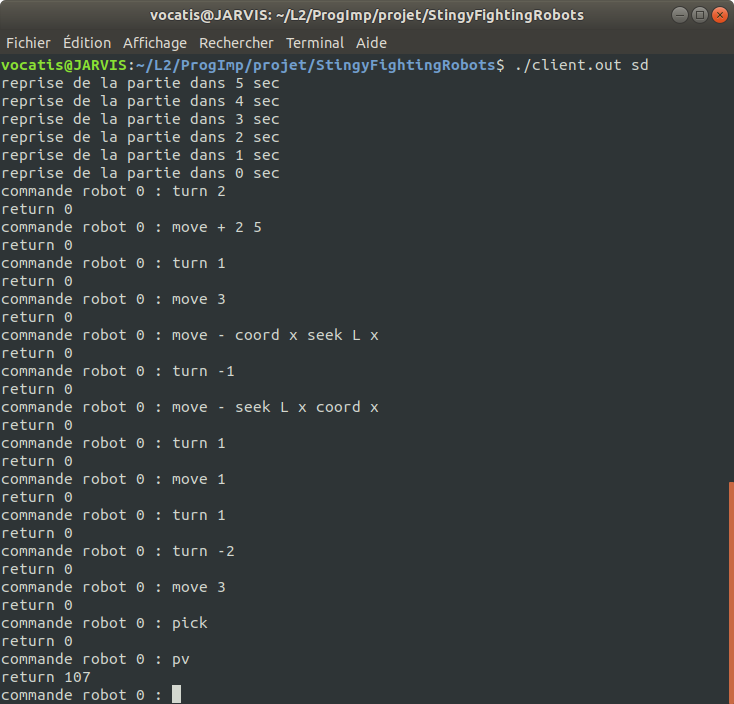
\includegraphics[scale=0.3]{utilisation_console.png}\\\\
Terminal affichant l'aire de jeu lors d'un échange de tirs entre deux robots\\\\
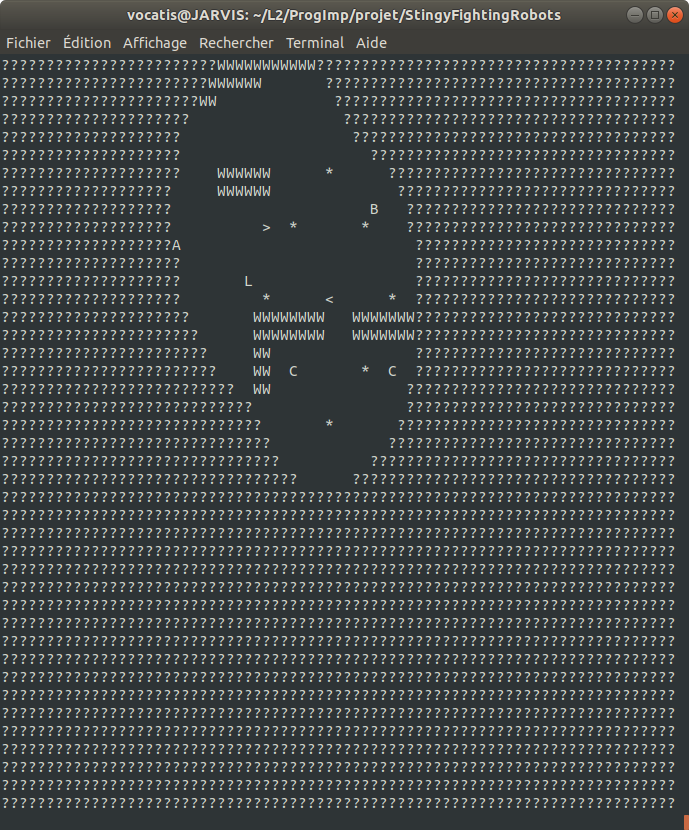
\includegraphics[scale=0.3]{exemple_de_tir.png}

\newpage
\appendix
\section{Code complet}
\subsection{Les déclarations}
\lstinputlisting[language=c]{../game.h}

\newpage
\subsection{Fonctions utilitaires}
\lstinputlisting[language=c]{../game.c}

\newpage
\subsection{Le client}
\lstinputlisting[language=c]{../client.c}

\newpage
\subsection{Le serveur}
\lstinputlisting[language=c]{../server.c}

\newpage
\subsection{Les fonctions minimalistes}
\lstinputlisting[language=c]{../fct_mini.c}

\newpage
\subsection{L'interpréteur}
\lstinputlisting[language=c]{../interpreteur.c}

\end{document}
